\documentclass[letterpaper, 11pt]{article}
\usepackage[utf8]{inputenc}
\usepackage[letterpaper, portrait, margin=1in]{geometry}
\usepackage{pgfplots}
\pgfplotsset{width=10cm,compat=1.9}
\usepackage{hyperref}
\usepackage{textcomp}
\usepackage{siunitx}
\usepackage{amsmath}
\usepackage{cancel}
\usepackage{tikz}
\usepackage{everysel}
\usepackage{ragged2e}
\usepackage{mathdots}
\usepackage{yhmath}
\usepackage{color}
\usepackage{array}
\usepackage{multirow}
\usepackage{amssymb}
\usepackage{gensymb}
\usepackage{tabularx}
\usepackage{booktabs}
\usetikzlibrary{fadings}
\usetikzlibrary{patterns}
\usetikzlibrary{shadows.blur}
\hypersetup{
    colorlinks=true,
    linkcolor=black,
    filecolor=black,      
    urlcolor=blue,
}

\title{COMSC-165 \\ Programming Assignment 8}
\author{Ryan Jacoby}
\date{15 July 2020}
\begin{document}

\maketitle

\section*{Run 1}
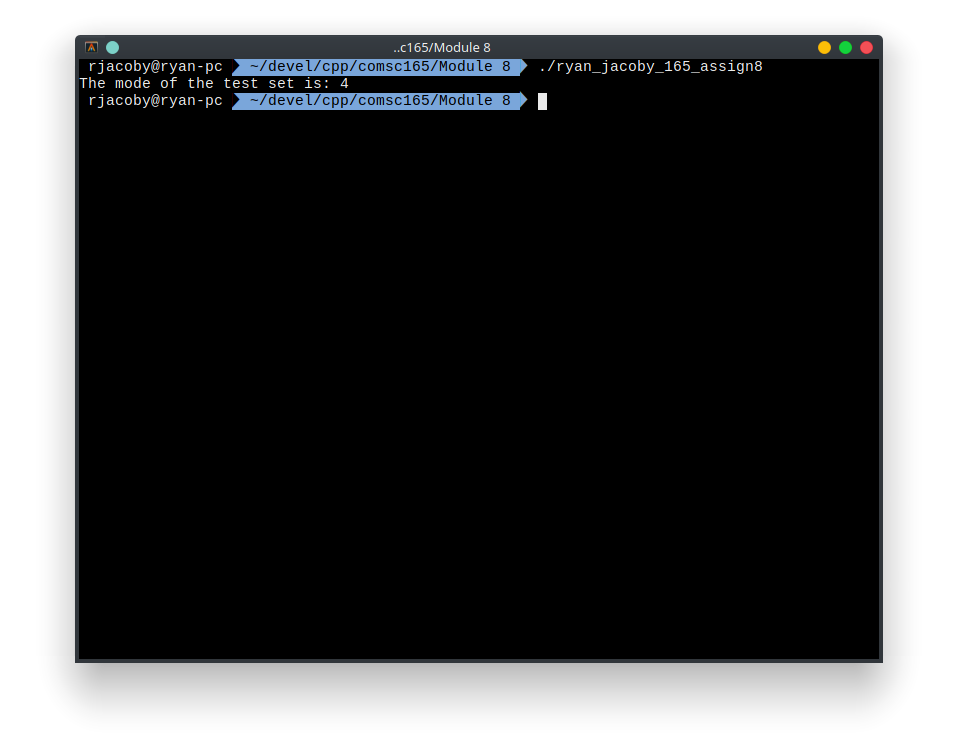
\includegraphics[scale=0.5]{run1.png} \\
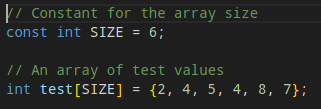
\includegraphics[scale=0.5]{run1_2.png}

\section*{Run 2}
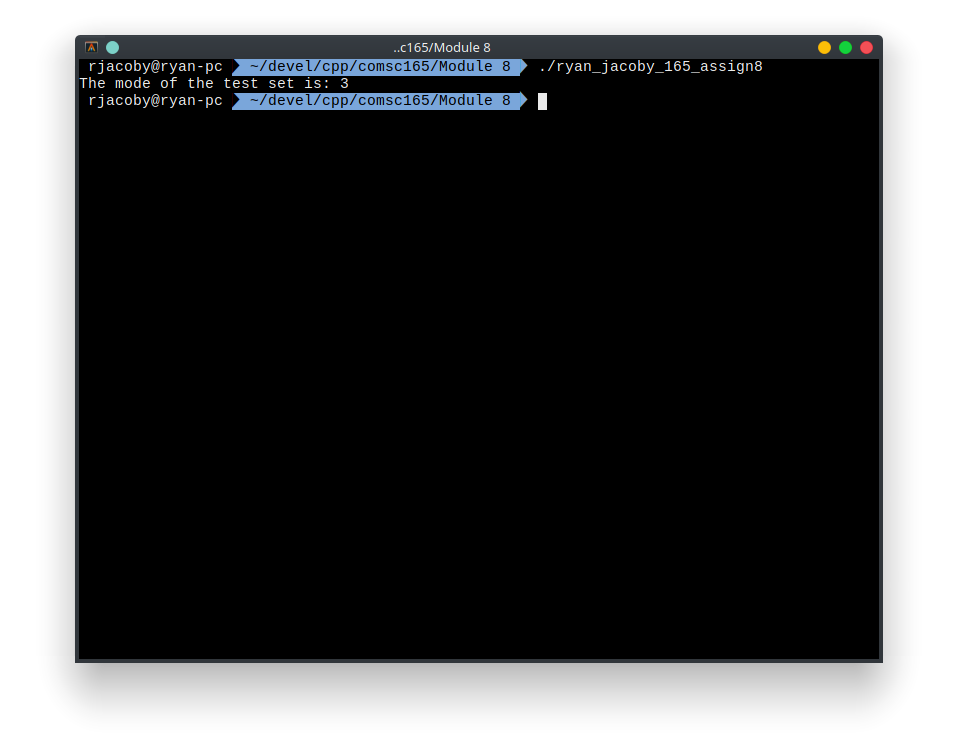
\includegraphics[scale=0.5]{run2.png} \\
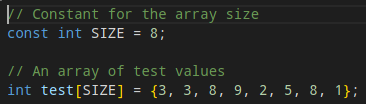
\includegraphics[scale=0.5]{run2_2.png}

\section*{Run 3}
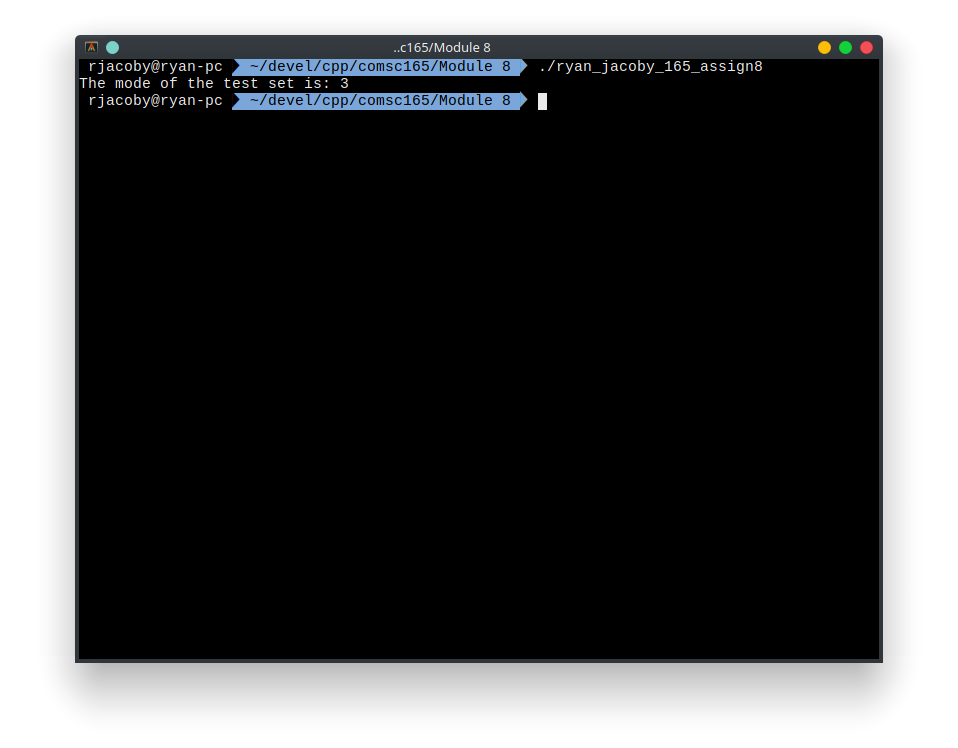
\includegraphics[scale=0.5]{run3.png} \\
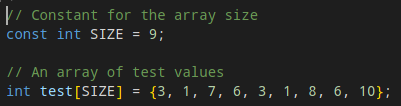
\includegraphics[scale=0.5]{run3_2.png}

\section*{Run 4}
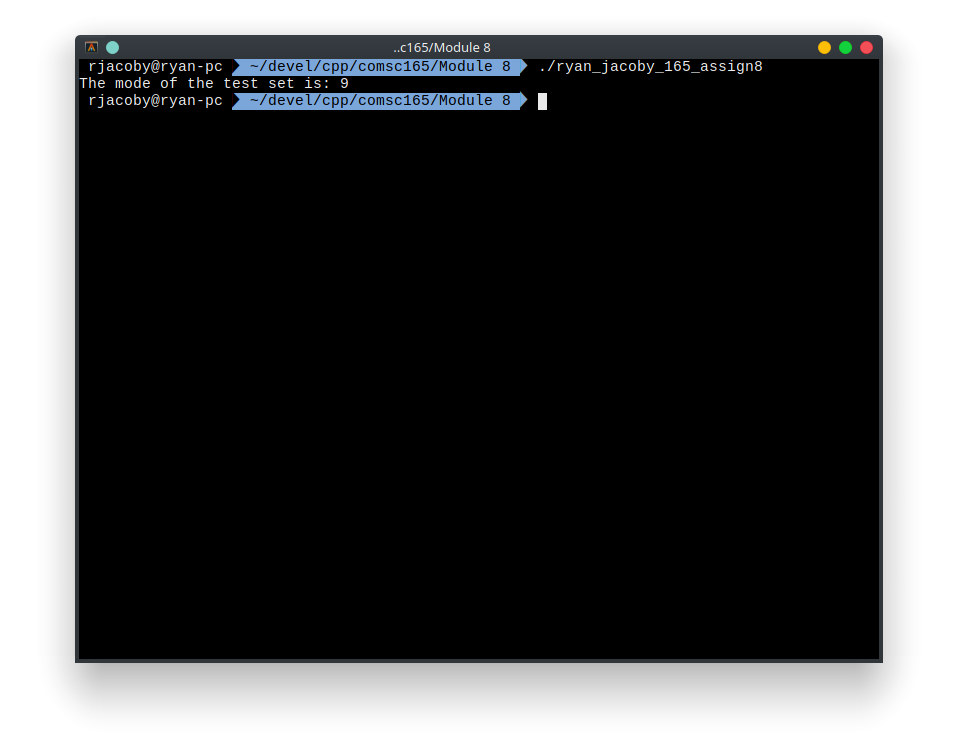
\includegraphics[scale=0.5]{run4.png} \\
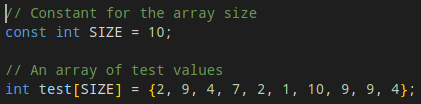
\includegraphics[scale=0.5]{run4_2.png}

\section*{Run 5}
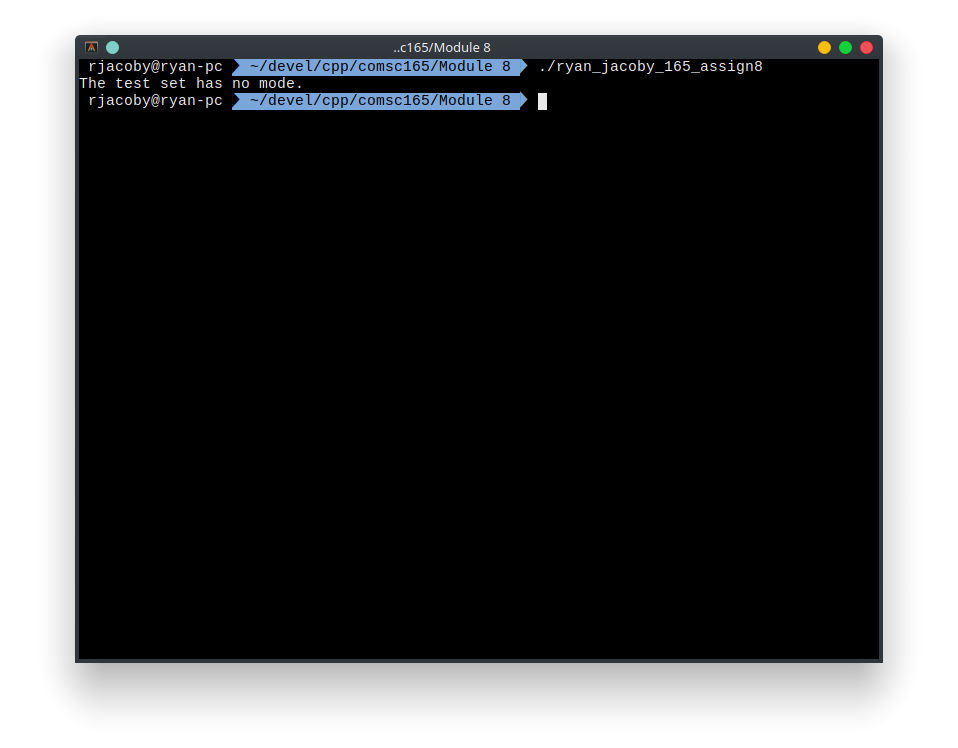
\includegraphics[scale=0.5]{run5.png} \\
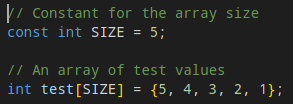
\includegraphics[scale=0.5]{run5_2.png}

\end{document}
